\documentclass[12pt]{article}

\usepackage{graphicx}
\usepackage{tikz}

\title{AMath Tea Time --- Puzzle \#2}
\author{}
\date{\vspace{-1cm}7 April 2015}

\begin{document}

\maketitle
\pagenumbering{gobble}

\subsection*{Problem}

Sherlock and Mycroft are playing Battleship on a $4 \times 4$ grid. Mycroft
hides a single $3 \times 1$ cruiser somewhere on the board. Sherlock can pick
squares on the grid and fire upon them. What is the smallest number of shots
Sherlock has to fire to guarantee at least one hit on the cruiser? {\it (Be sure
  to prove that fewer shots than this number will not work!)}

\begin{figure}[h]
  \centering
  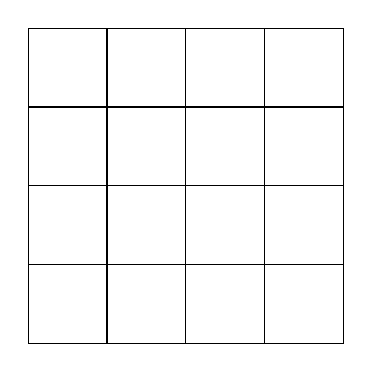
\begin{tikzpicture}[scale=1]
    \draw (0,0) -- (4,0) -- (4,4) -- (0,4) -- (0,0);
    \draw (1,0) -- (1,4);
    \draw (2,0) -- (2,4);
    \draw (3,0) -- (3,4);
    \draw (0,1) -- (4,1);
    \draw (0,2) -- (4,2);
    \draw (0,3) -- (4,3);
    \end{tikzpicture}
\end{figure}

\subsection*{Hints}

{\it (Posted on Thursday)}


{
\par\vspace*{\fill}
\noindent \small \it
If you have any puzzles to share then send them my way at {\tt
  cswiercz@uw.edu}!
}

\end{document}
